% THIS IS SIGPROC-SP.TEX - VERSION 3.1
% WORKS WITH V3.2SP OF ACM_PROC_ARTICLE-SP.CLS
% APRIL 2009
%
% It is an example file showing how to use the 'acm_proc_article-sp.cls' V3.2SP
% LaTeX2e document class file for Conference Proceedings submissions.
% ----------------------------------------------------------------------------------------------------------------
% This .tex file (and associated .cls V3.2SP) *DOES NOT* produce:
%       1) The Permission Statement
%       2) The Conference (location) Info information
%       3) The Copyright Line with ACM data
%       4) Page numbering
% ---------------------------------------------------------------------------------------------------------------
% It is an example which *does* use the .bib file (from which the .bbl file
% is produced).
% REMEMBER HOWEVER: After having produced the .bbl file,
% and prior to final submission,
% you need to 'insert'  your .bbl file into your source .tex file so as to provide
% ONE 'self-contained' source file.
%
% Questions regarding SIGS should be sent to
% Adrienne Griscti ---> griscti@acm.org
%
% Questions/suggestions regarding the guidelines, .tex and .cls files, etc. to
% Gerald Murray ---> murray@hq.acm.org
%
% For tracking purposes - this is V3.1SP - APRIL 2009

\documentclass{acm_proc_article-sp}

\begin{document}

\title{Image Retrieval Using Visual Words and Spatial Re-ranking}
\subtitle{Project of Visual Data Retrieval and Detection}
%
% You need the command \numberofauthors to handle the 'placement
% and alignment' of the authors beneath the title.
%
% For aesthetic reasons, we recommend 'three authors at a time'
% i.e. three 'name/affiliation blocks' be placed beneath the title.
%
% NOTE: You are NOT restricted in how many 'rows' of
% "name/affiliations" may appear. We just ask that you restrict
% the number of 'columns' to three.
%
% Because of the available 'opening page real-estate'
% we ask you to refrain from putting more than six authors
% (two rows with three columns) beneath the article title.
% More than six makes the first-page appear very cluttered indeed.
%
% Use the \alignauthor commands to handle the names
% and affiliations for an 'aesthetic maximum' of six authors.
% Add names, affiliations, addresses for
% the seventh etc. author(s) as the argument for the
% \additionalauthors command.
% These 'additional authors' will be output/set for you
% without further effort on your part as the last section in
% the body of your article BEFORE References or any Appendices.

\numberofauthors{3} %  in this sample file, there are a *total*
% of EIGHT authors. SIX appear on the 'first-page' (for formatting
% reasons) and the remaining two appear in the \additionalauthors section.
%
\author{
% You can go ahead and credit any number of authors here,
% e.g. one 'row of three' or two rows (consisting of one row of three
% and a second row of one, two or three).
%
% The command \alignauthor (no curly braces needed) should
% precede each author name, affiliation/snail-mail address and
% e-mail address. Additionally, tag each line of
% affiliation/address with \affaddr, and tag the
% e-mail address with \email.
%
% 1st. author
\alignauthor Ke Lin\titlenote{This author do some experiments and revise paper}\\
       \affaddr{School of Software }\\
       \affaddr{Tsinghua University}\\
       \affaddr{Beijing, China}\\
       \email{linke0113@gmail.com}
% 2nd. author
\alignauthor Chen Chen\titlenote{This author do some experiments and revise paper}\\
       \affaddr{School of Software }\\
       \affaddr{Tsinghua University}\\
       \affaddr{Beijing, China}\\
       \email{chenchen\_9207@163.com}
% 3rd. author
\alignauthor Qingfu Wen\titlenote{This author write code, do some experiments and write paper}\\
       \affaddr{School of Software }\\
       \affaddr{Tsinghua University}\\
       \affaddr{Beijing, China}\\
       \email{thssvince@163.com}
}
% There's nothing stopping you putting the seventh, eighth, etc.
% author on the opening page (as the 'third row') but we ask,
% for aesthetic reasons that you place these 'additional authors'
% in the \additional authors block, viz.
\date{12 December 2014}
% Just remember to make sure that the TOTAL number of authors
% is the number that will appear on the first page PLUS the
% number that will appear in the \additionalauthors section.

\maketitle
\begin{abstract}
The ``bag of words"(BoW) model is very popular in large-scale text retrieval and image retrieval. SIFT descriptor is also wildly used in large scale image retrieval. In this paper, we implement an image retrieval algorithm based on SIFT and BoW. Traditionally, we can obtain an ordered list of top N images from the dataset which have the highest relevance to each query instance. However, the performance of naive BoW method is not ideal because it lacks spatial information. In this paper, we perform a spatial re-ranking on the ordered list to recalculate the similarity between each image and the query instance. In our experiments based on the \textbf{Oxford 5K} dataset, we can utilize spatial verification to achieve better retrieval accuracy at manageable computational cost.
\end{abstract}

\terms{Algorithms}
\keywords{Image Retrieval, SIFT, Bag of Words, Spatial Re-ranking} % NOT required for Proceedings

\section{Introduction}
Along with the fast increasing of image data, large-scale image retrieval has becoming more and more significant in both academia
and industry. The problem of searching images according to their semantic content, which is also called content-based image retrieval (CBIR), is very challenging since many factors can affect the performance of CBIR, like resolution, illumination variations and occluded objects.\par

Albeit global features like colors, textures, and shapes have been used to represent images, they still have a plethora of  limits. Scale Invariant Feature Transform (SIFT)\cite{aLowe:Object} was proposed for describing several salient patches around key points within the images. Based on this local descriptor vectors, a popular approach, bag-of-words (BoW), was proposed in \cite{bSivic:Video}. It is noted that the BoW approach, although is simple and directly borrowed from text retrieval community, has shown excellent performance not only for CBIR task but also for other vision tasks like object recognition, image classification and annotation.
\section{SIFT \& BoW}
\subsection{SIFT}
SIFT features demonstrating great discriminative power are invariant to the changes of rotation, scaling, translation and distortions. SIFT descriptor can be extracted in the following 4 steps.
\begin{itemize}
\item Construct scale space, test interest points and get scale invariant feature.
\begin{figure}[h]
\centering
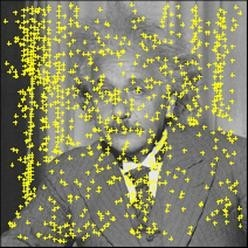
\includegraphics[height=4cm ,width=4cm,angle=0]{sift1.jpg}
\end{figure}

\item eliminate unstable points.
\begin{figure}[h]
\centering
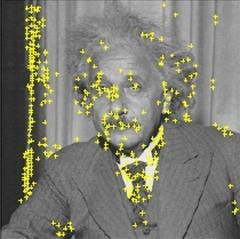
\includegraphics[height=4cm ,width=4cm,angle=0]{sift2.jpg}
\end{figure}

\item obtain orientation for each key point.
\begin{figure}[h]
\centering
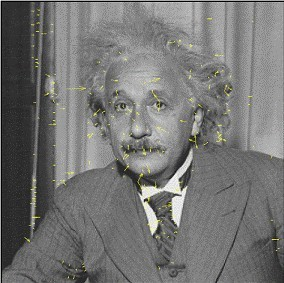
\includegraphics[height=3.5cm ,width=3.5cm,angle=0]{sift3.jpg}
\end{figure}

\item generate a 128-D descriptor for each point.
\begin{figure}[h]
\centering
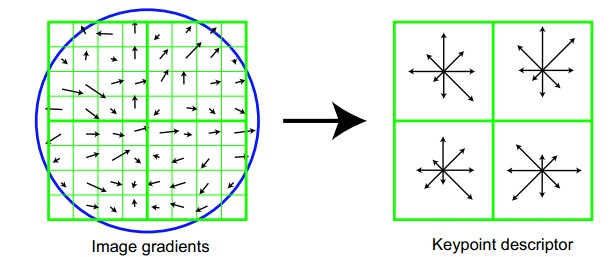
\includegraphics[height=2.5cm ,width=6cm,angle=0]{sift4.jpg}
\end{figure}
\end{itemize}
After these steps, we can gain a 128$\times$n descriptor for each image.
\subsection{BoW}
BoW model is a very common method in information retrieval. We will use an example to demonstrate BoW in image retrieval. For example, there are 3 categories of images--face, bike and guitar.\par
The first step of BoW is to extract SIFT features and extract visual words from all the images.\par
\begin{figure}[h!]
\centering
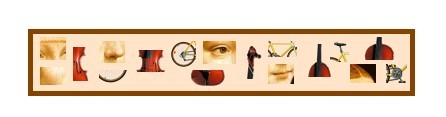
\includegraphics[height=1.5cm ,width=6cm,angle=0]{bow1.jpg}
\end{figure}

Second, generate word list using K-Means.\par
\begin{figure}[h!]
\centering
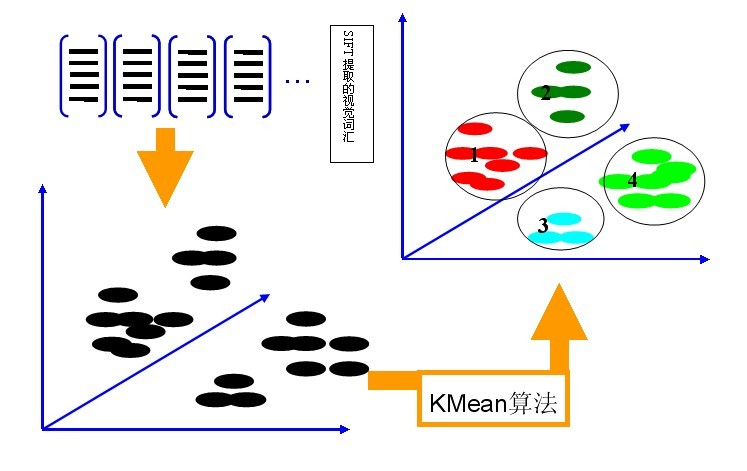
\includegraphics[height=5cm ,width=5cm,angle=0]{bow2.jpg}
\end{figure}


Finally, map each image to the word list. We can use a word list to represent an image.
\begin{figure}[h!]
\centering
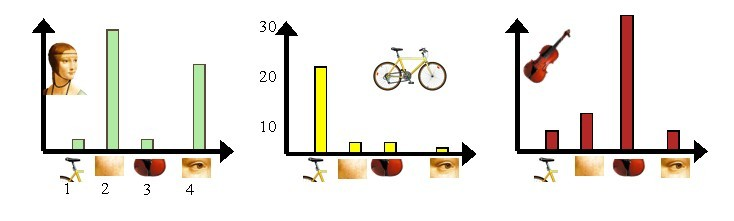
\includegraphics[height=2.3cm ,width=8cm,angle=0]{bow3.jpg}
\end{figure}

\section{Dataset}
The entire dataset consists of 5,062 high resolution (1024$\times$768) images, comprising 11 different Oxford ``landmarks" - a particular part of a building. Sample images from the dataset are shown in figure 1.
\begin{figure}
\centering
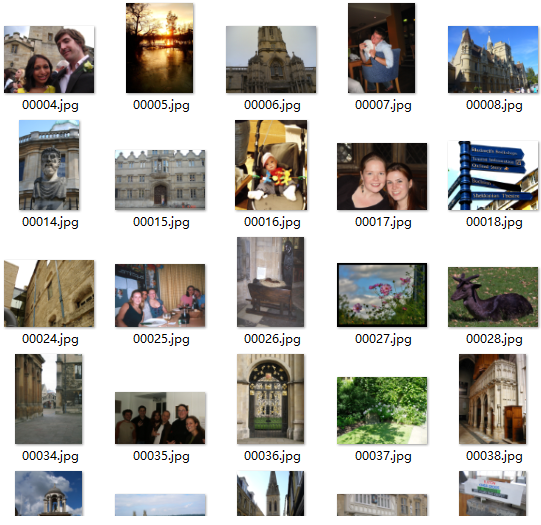
\includegraphics[height=6.18cm ,width=6cm,angle=0]{dataset.png}
\caption{Randomly sampled images from the 5K dataset. Note
that the dataset contains difficult distractors which may easily be
confused with those used in the query set.}
\end{figure}
\section{Implementatioin}
We implement this experiment using VLFeat\footnote{http://www.vlfeat.org/} in MATLAB on Windows Server 2008 with 32G memory and 16-core CPU.
\subsection{Extract SIFT features}
For each image in the dataset, we can extract about 3000 128-D SIFT descriptors.
\subsection{Generate visual vocabularies}
In previous step, we may obtain about 15M SIFT descriptors. We perform a K-Means clustering on these descriptors with K = 100000. Then we can 100000-D visual vocabulary for all the image words.
\subsection{Describe image width visual vocabulary}
We try to assign each image to the 100000-D vocabulary using KD-Tree. Normally, we can use a 100000-dimension vector to describe each image.
\subsection{Query}
In this stage, we can naturally assign a query image to a 100000-D vector. Now, we compute the distance\footnote{the number of words both appears in image A and image B} between a query image and each image in dataset. we sort the list to get top-N images by distance.
\subsection{Re-rank}
At last, we try to re-rank this top-N list using Spatial information. We try to match the query instance and dataset images with SIFT again. Experimental results show higher accuracy after this step.

\section{Results}
We run this experiment twice for comparison. First, we run it without re-ranking. You can see the mAP of each category in table 1. Second, we run it again to gain top 100 images with re-ranking. Results show in table 2.
\begin{table}
\centering
\begin{tabular}{|c|c|c|c|c|c|} \hline
Category    & top100 & top200 & top400 & top800 & top1000\\ \hline
all\_souls  & 0.2594 & 0.2830 & 0.3025 & 0.3137 & 0.3161\\ \hline
ashmolean   & 0.1863 & 0.1888 & 0.1906 & 0.1925 & 0.1929\\ \hline
balliol     & 0.1911 & 0.1956 & 0.1962 & 0.1970 & 0.1974\\ \hline
bodleian    & 0.5620 & 0.5677 & 0.5713 & 0.5722 & 0.5728\\ \hline
chris\_chur  & 0.4197 & 0.4449 & 0.4587 & 0.4629 & 0.4641\\ \hline
cornmarket  & 0.3179 & 0.3190 & 0.3206 & 0.3223 & 0.3227\\ \hline
mAP         & \textbf{0.3227} & \textbf{0.3397} & \textbf{0.3400} & \textbf{0.3434} & \textbf{0.3443}\\ \hline
\end{tabular}
\caption{Average precision without re-ranking}
\end{table}

\begin{table}
\centering
\begin{tabular}{|c|c|c|} \hline
Category    & no re-ranking & re-ranking \\ \hline
all\_souls\_1  & 0.0543 & 0.0883 \\ \hline
all\_souls\_2  & 0.2514 & 0.3009 \\ \hline
all\_souls\_3  & 0.2269 & 0.2919 \\ \hline
all\_souls\_4  & 0.3974 & 0.4913 \\ \hline
all\_souls\_5  & 0.3672 & 0.5158 \\ \hline
ashmolean\_1   & 0.0780 & 0.2029 \\ \hline
ashmolean\_2   & 0.3009 & 0.4768 \\ \hline
ashmolean\_3   & 0.0421 & 0.0883 \\ \hline
ashmolean\_4   & 0.1938 & 0.2328\\ \hline
ashmolean\_5   & 0.3167 & 0.4202\\ \hline
balliol\_1     & 0.3483 & 0.6784\\ \hline
balliol\_2     & 0.1200 & 0.1855\\ \hline
balliol\_3     & 0.1362 & 0.3333\\ \hline
balliol\_4     & 0.1075 & 0.3333\\ \hline
balliol\_5     & 0.2433 & 0.5470\\ \hline
bodleian\_1    & 0.6158 & 0.6429\\ \hline
bodleian\_2    & 0.0491 & 0.2083\\ \hline
bodleian\_3    & 0.3488 & 0.5112\\ \hline
bodleian\_4    & 0.8921 & 0.9479\\ \hline
bodleian\_5    & 0.9044 & 0.8770\\ \hline
christ\_church\_1  & 0.5318 & 0.6517\\ \hline
christ\_church\_2  & 0.5919 & 0.6745\\ \hline
christ\_church\_3  & 0.5014 & 0.6044\\ \hline
christ\_church\_4  & 0.4287 & 0.5379\\ \hline
christ\_church\_5  & 0.0448 & 0.1026\\ \hline
cornmarket\_1  & 0.4593 &  0.5556\\ \hline
cornmarket\_2  & 0.1128 &  0.2222\\ \hline
cornmarket\_3  & 0.4554 &  0.5556\\ \hline
cornmarket\_4  & 0.2286 &  0.3333\\ \hline
cornmarket\_5  & 0.3333 &  0.4444\\ \hline
mAP         & \textbf{0.3227} & \textbf{0.4352}\\ \hline
\end{tabular}
\caption{Average precision @top100}
\end{table}


\section{Conclusions and further work}
We try to demonstrate a framework for image retrieval using SIFT and BoW with re-ranking. From the experimental results, we can see pretty good performance but not perfect. Unfortunately, because of the limitation of time, we did not pay much attention on the K-Means step. A more accurate K-Means algorithm may perform a better result in retrieval, like Approximate K-Means\cite{cPhilbin07:Object}. Meanwhile, the re-ranking stage has much work to research\cite{d658:Hough}.

%ACKNOWLEDGMENTS are optional
\section{Acknowledgments}
We are grateful to Prof. Guiguang Ding who taught us a lot of useful visual data processing and analysis methods. In addition, thanks to our TA, Shijiang Chen, who provided us with guidance materials, we can finish our project successfully. Finally, thank you for reading this paper written in our poor English.

\bibliographystyle{abbrv}
\bibliography{sigproc}  % sigproc.bib is the name of the Bibliography in this case
\end{document}
